%% Fall 2013 MDM Homework Template
\documentclass[12pt,letterpaper]{article}

\usepackage[utf8]{inputenc}
\usepackage[T1]{fontenc}
\usepackage{amsmath}
\usepackage{amsfonts}
\usepackage{amssymb}
\usepackage[left=2cm,right=2cm,top=2cm,bottom=2cm,headheight=22pt]{geometry}
\usepackage{fancyhdr}
\usepackage{setspace}
\usepackage{lastpage}
\usepackage{graphicx,subcaption}
\usepackage{tikz}

\begin{document}

%other parameters
\setlength{\parskip}{1ex plus 0.5ex minus 0.2ex}
\setlength{\parindent}{0pt}

%header and footer parameters
\pagestyle{fancy}
\lhead{Math 1100}
\chead{Weekly Homework}
\rhead{Due: April 29}
\lfoot{}
\cfoot{\emph{Prof. Hitchman}}
\rfoot{}

\begin{center}
{
\Large
\textbf{Cantor: Assignment \#4}
}
\end{center}

\section*{Specifications for Grading}

To earn credit, this assignment must
\begin{itemize}
\item be typed, of no more than one or two pages in length;
\item address one of the tasks below;
\item conform to reasonable standards for grammar, spelling, and usage of the English language with minimal errors. (You may consider seeking help on writing from the Writing Center in the Academic Learning Center. http://www.uni.edu/unialc/writing-center);
\item be turned in by 3pm on Friday, April 29.
\end{itemize}


\textbf{For this Assignment, you may do either one these two tasks. You must do one. You may do both.}


\subsection*{Task One}

Suppose that you are given two sets $A$ and $B$.
At this point, the names are just place holders. 
These sets could be just about anything!
Well, not \emph{anything}.
You know for sure that both $A$ and $B$ are countably infinite.\\

Show that there is a matching between the elements of $A$ and the elements of $B$.
That is, describe how you know there has to be such a matching, and how you would go about sharing that matching.

Write as if describing this to a friend who is not in this class, but could be.

\vfill

{\small Turn over for the second task.}

\clearpage
\subsection*{Task Two}


Two friends argue over the number of points on two circles: one small, one large.
Here is their argument.

Friend number 1 says:
\begin{quote}
Say the circles are concentric. 
Every ray you draw from the center of the circles will cut the big circle once and the little circle once. 
This makes a correspondence between the points of the one circle and the points of the other circle.
So they have the same amount of points.
\end{quote}

Friend number 2 then says:
\begin{quotation}
Okay, let's take concentric circles. Draw a horizontal line through the center.
I want to move this line up and down, but keep it parallel to the original position.
At first, the line cuts both circles in two places. 
That looks like a way to make the points correspond.
But as you get far enough, the line will cut the big circle twice, but only just touch the smaller circle at one point. 
And if you get farther away than that, the line will touch the bigger circle (still twice!), but not touch the little circle at all.

Therefore, all points on the smaller circle are related to some point on the bigger one, but some points on the bigger one are not related to point on the smaller one.
So the larger circle has more points.
\end{quotation}

How can we make sense of what is going on here? Say which friend is correct, and why. Say where the other friend is making a subtle mistake.
\vspace{.1cm}
\begin{center}
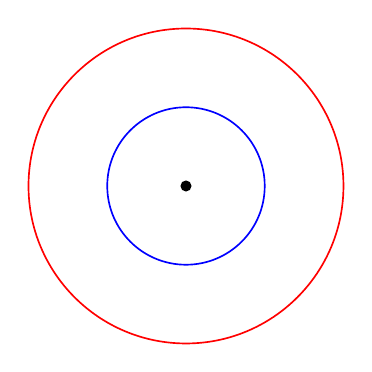
\begin{tikzpicture}
    \draw[blue,semithick] (0,0) circle (1cm);
    \draw[red,semithick] (0,0) circle (2cm);
    \fill  (0,0) circle [radius=2pt];
\end{tikzpicture}
\end{center}




\end{document}
%sagemathcloud={"zoom_width":100}